\chapter{Introduction}
\label{chap:intro}
\lhead{\emph{Introduction}}
This project aims to create an automated Docker linter tool to improve the security, efficiency and maintainability of Docker images. This will be done by analysing the dockerfiles and looking for docker smells within the file.It will also force developers to follow best practices within the docker file by using preset rules.This linter helps developers with workflow and will streamline the Devops team by using the \textit{shift-left} approach. 
This tool combines two main functionalities : 
\begin{enumerate}
    \item Docker Linting for best practices:
    The Linter performs static analysis of Dockerfiles to ensure that they meet the best practices and rules.This includes detecting issues such as using outdated or large base images, running containers as root, exposing unnecessary ports, etc.
    \item Docker Smells Detection: The linter also identifies \textit{Docker Smells} - poor practices in Dockerfiles.This can cause security issues, bloating, and inefficiency. 
    By identifying these issues early on, it will lead to a more secure and smaller image. The linter will check which smells are most frequently fixed within the industry and advice the developer if it is worth fixing or not. 
\begin{figure}[ht]
  \centering
  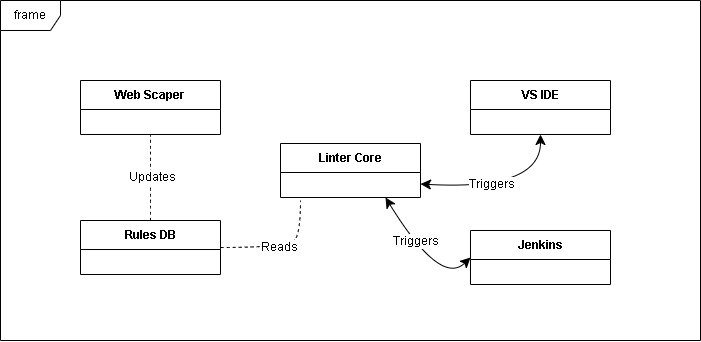
\includegraphics[width=0.63\textwidth]{UML.png}
  \caption{High Level Overview} % Use braces {} for the caption text
  \label{fig:Overview1} % Ensure unique label
\end{figure}
\end{enumerate}

\section{Motivation}
The concept for this project initially came to mind while I was interning as a Software Security Engineer at IBM.When I was at IBM, I learned about containerisation. Specifically, he delved into Docker and Kubernetes.At the beginning of my internship, he had a discussion with a developer who had knowledge of Kubernetes and Docker images.I was taken aback when he mentioned that he needed to inspect dockerfiles to ensure they followed practices and satisfied specific security criteria.

Performing manual check of Dockerfiles to spot security vulnerabilities and inefficiencies as poor practices appeared to be a task-prone, error-prone, and time-consuming effort, particularly in extensive setups where many Docker images are deployed. It introduces complexities into the development flow but also raises the likelihood of human mistakes. Reflectively thinking back to that discussion made me recognise a need for enhancing the automation of Dockerfile assessments with a focus on ensuring security compliance and streamlining Dockerfile optimisation. 

Fascinated by this issue, I delved into exploring solutions that already existed and found out about the availability of Docker linting tools. As an example, Red Hat had created a Docker lint tool to automate some of these validations. Unfortunately, the project has been discontinued. The abandonment of such a tool in this field further emphasised the necessity for a solution that could be embraced by developers on a large scale. 

In my exploration of the topic at hand, I came across the idea of "Docker Smells," which are essentially bad practices found in Dockerfiles that can result in inefficient or insecure images that are hard to maintain.Some "Docker smells" may be insignificant or only affect the appearance of the code slightly; however, others could potentially cause performance or security problems.This discovery inspired me to create a tool that not only promotes practices but also assesses whether addressing Docker smells is necessary.This tool provides insights into which issues are crucial to resolve and which ones can be overlooked. 

By developing a Docker linter that includes these features, I intend to assist developers in managing their workload and simplifying their workflow by decreasing tasks and increasing security through issue detection.Automating these validations can enhance efficiency by reducing image size, securing configurations, and encouraging teams to adhere to practices.Teams working in high-speed environments where even small mistakes in Dockerfiles could cause problems will find this tool especially helpful.

In essence, I am driven to work on this project because I want to connect containerization with security automation and effectively create a tool that addresses the increased demand, for improved tools in the container environment space.This project reflects not my fascination with DevOps and security but also my dedication, to solving practical challenges that developers encounter in their daily tasks.  


\section{Contribution}
This project reflects a culmination of key skills and knowledge I have developed during my studies in Computer systems. The Docker linter leverages several core concepts, particularly in software development, security, and automation. Through modules like \textit{Object Orientated Programming}, \textit{Operating Systems} and \textit{Agile Processes}, I developed a deep understanding of containerisation technologies, including Docker, which forms the backbone of this project. The Linter automates the enforcement of best practices for Dockerfiles, helping developers optimise their container builds by reducing security risks, improving efficiency, and maintaining consistency.

One of the most significant contributions of this project is its focus on security. By using  modules like \textit{Network Fundamentals} and \textit{Linux Administration}, I applied best practices to ensure that the Docker linter can detect security vulnerabilities such as the use of outdated base images, running containers as root, and exposing unnecessary ports. Automating these checks helps developers adhere to  security practices earlier in their development process, aligning with the "shift-left" security philosophy that I encountered during my internship at IBM.

Furthermore, this project goes beyond standard Dockerfile linting by incorporating the analysis of \textit{Docker smells} anti-patterns that downgrade the performance and maintainability of containerised applications. My linter not only identifies these smells but also prioritises which issues are worth fixing, offering developers actionable insights to improve their Dockerfiles. This aspect of the project demonstrates both innovation and problem-solving, showcasing my ability to extend traditional solutions to meet modern software engineering needs.

In summary, this project reflects my ability to apply computer systems knowledge in a practical setting, integrating concepts such as static code analysis, DevOps practices, and security automation. It bridges academic theory with real-world application, ensuring that the skills I have acquired are used to solve meaningful problems in the area of containerised software development.

\section{Structure of This Document}
% notice how I cross referenced the chapters through using the \label tag --> LaTeX is VERY similar to HTML and other mark up languages so you should see nothing new here!
\textit{Chapter One} is a detailed introduction to the project.It gives a high overview with the aid of a diagram,discuses the motivation behind the idea, and the contribution this project may have on the industry in large. 
\textit{Chapter Two} discusses the core areas being met within computer science and determines what has been done within the industry.These areas are based on software engineering, Devops development, Cloud automation and containerisation, Docker security, and CI/CD automation. 
\textit{Chapter Three} talks about the problems within the industry that we are trying to solve as well the functional and non-functional requirements for this project.
\textit{Chapter Four} outlines the strategy for developing the Docker linter. It mentions the architecture, rick assessment,methodology and implementation plan for this project. 
\textit{Chapter Five} is the conclusion of the paper, where the project as well as any future work is discussed. 